%%%%%%%%%%%%%%%%%%%%%%%%%%%%%%%%%%%%%%%%%
% a0poster Portrait Poster
% LaTeX Template
% Version 1.0 (22/06/13)
%
% The a0poster class was created by:
% Gerlinde Kettl and Matthias Weiser (tex@kettl.de)
% 
% This template has been downloaded from:
% http://www.LaTeXTemplates.com
%
% License:
% CC BY-NC-SA 3.0 (http://creativecommons.org/licenses/by-nc-sa/3.0/)
%
%%%%%%%%%%%%%%%%%%%%%%%%%%%%%%%%%%%%%%%%%

%----------------------------------------------------------------------------------------
%	PACKAGES AND OTHER DOCUMENT CONFIGURATIONS
%----------------------------------------------------------------------------------------

\documentclass[a0,portrait]{a0poster}

\usepackage{multicol} % This is so we can have multiple columns of text side-by-side
\columnsep=100pt % This is the amount of white space between the columns in the poster
\columnseprule=3pt % This is the thickness of the black line between the columns in the poster

\usepackage[svgnames]{xcolor} % Specify colors by their 'svgnames', for a full list of all colors available see here: http://www.latextemplates.com/svgnames-colors

\usepackage{times} % Use the times font
%\usepackage{palatino} % Uncomment to use the Palatino font

\usepackage{graphicx} % Required for including images
\graphicspath{{figures/}} % Location of the graphics files
\usepackage{booktabs} % Top and bottom rules for table
\usepackage[font=small,labelfont=bf]{caption} % Required for specifying captions to tables and figures
\usepackage{amsfonts, amsmath, amsthm, amssymb} % For math fonts, symbols and environments
\usepackage{wrapfig} % Allows wrapping text around tables and figures
\usepackage{natbib}
\usepackage{color}
\usepackage[colorlinks=true,
            linkcolor=gray,
            urlcolor=black,
            citecolor=blue]{hyperref}
            
\usepackage{mathtools}
\usepackage{textgreek}
\usepackage{MnSymbol,wasysym}
\usepackage{ragged2e}
\usepackage{csvsimple}
\usepackage{color}
\usepackage{subfig}
\usepackage{titlesec}
\titlespacing\section{10pt}{12pt plus 4pt minus 2pt}{4pt plus 2pt minus 2pt}
\titlespacing\subsection{0pt}{12pt plus 4pt minus 2pt}{0pt plus 2pt minus 2pt}
\titlespacing\subsubsection{0pt}{12pt plus 4pt minus 2pt}{0pt plus 2pt minus 2pt}

\begin{document}

%----------------------------------------------------------------------------------------
%	POSTER HEADER 
%----------------------------------------------------------------------------------------

% The header is divided into two boxes:
% The first is 75% wide and houses the title, subtitle, names, university/organization and contact information
% The second is 25% wide and houses a logo for your university/organization or a photo of you
% The widths of these boxes can be easily edited to accommodate your content as you see fit

\begin{minipage}[b]{0.75\linewidth}
\veryHuge \color{NavyBlue} \textbf{Efficient mode jumping MCMC for Bayesian\\ variable selection in GLMM} \color{Black}\\[1cm] % Title
\Huge\textit{Nord Stat 2016, June 27-30, 2016 Copenhagen, Denmark}\\[2cm] % Subtitle
\huge \textbf{Aliaksandr Hubin \& Geir Storvik}\\[0.5cm] % Author(s)
\huge Department of Mathematics, University of Oslo\\[0.4cm] % University/organization
\Large \texttt{aliaksah@math.uio.no, geirs@math.uio.no}\\
\end{minipage}
%
\begin{minipage}[b]{0.75\linewidth}

\includegraphics[width=25cm]{logo.jpg}\\
 \hspace*{5cm}
\includegraphics[width=3cm]{cels.png} \hspace{2cm}

\includegraphics[width=7cm]{qrcode.png}\\
\end{minipage}

%\vspace{1cm} % A bit of extra whitespace between the header and poster content

%----------------------------------------------------------------------------------------

\begin{multicols}{2} % This is how many columns your poster will be broken into, a portrait poster is generally split into 2 columns

%----------------------------------------------------------------------------------------
%	ABSTRACT
%----------------------------------------------------------------------------------------

\color{Navy} % Navy color for the abstract

\begin{abstract}


Generalized linear mixed models (GLMM) are addressed for inference and prediction in a wide range of different applications providing a powerful scientific tool for the researchers and analysts coming from different fields. At the same time more sources of data are becoming available introducing a variety of hypothetical explanatory variables for these models to be considered. Estimation of posterior model probabilities and selection of an optimal model is thus becoming crucial. We suggest a novel mode jumping MCMC procedure for Bayesian model averaging and model selection in GLMM.

\end{abstract}

%----------------------------------------------------------------------------------------
%	INTRODUCTION
%----------------------------------------------------------------------------------------

\color{SaddleBrown} % SaddleBrown color for the introduction

\section*{Introduction}

In this study we address variable selection in generalized linear mixed models (GLMM) addressed in the Bayesian setting. These models allow to carry out detailed modeling in terms of both linking reasonably chosen responses and explanatory variables via a proper link function and incorporating the unexplained variability and dependence structure between the observations via random effects. Being one of the most powerful modeling tools in modern statistical science GLMM models have proven to be efficient in numerous applications from banking to astrophysics and genetics \cite{Hubin2016}. The posterior distribution of the models  can be viewed as a  relevant measure for the model evidence, based on the observed data. The number of models to select from is exponential in the number of candidate variables, moreover the search space in this context is often extremely non-concave. Hence efficient search algorithms have to be adopted for evaluating the posterior distribution of models within a reasonable amount of time. In this paper we introduce efficient mode jumping MCMC algorithms for calculating and maximizing posterior probabilities of the GLMM models. 

%----------------------------------------------------------------------------------------
%	OBJECTIVES
%----------------------------------------------------------------------------------------

\color{DarkSlateGray} % DarkSlateGray color for the rest of the content

\section*{Model and Inference}

Generalized linear mixed models consist of a response $Y_{t}$ coming from the exponential family distribution, a vector of $P$ variables $X_{ti}$ for observations $t \in \{1,...,T\}$ and latent indicators $\gamma_i\in\{0,1\}, i \in \{1,...,P\}$ defining if variable $X_{ti}$ is  included into the model ($\gamma_i = 1$) or not ($\gamma_i = 0$). We are also addressing the unexplained variability of the responses and the correlation structure between them through random effects $\delta_t$ with a specified parametric and sparse covariance matrix structure. Conditioning on the random effect we model the dependence of the responses on the explanatory variables via a proper link function $g(\cdot)$:
\begin{eqnarray} \label{themodeleq}
  &Y_t|\mu_t \sim  \mathfrak{f}(y|\mu_t)\\
  &g(\mu_t) =   \beta_0 + \sum_{i=1}^{P} \gamma_i\beta_{i}X_{ti} + \delta_t\\
 &\boldsymbol{\delta} = (\delta_1,...,\delta_T) \sim N_T\left(\boldsymbol{0},\boldsymbol{\Sigma}_b\right).\label{themodeleqend}
\end{eqnarray}
Here $\beta_i \in \mathbb{R}, i \in \{0,...,P\}$ are regression coefficients showing in which way variables influence the linear predictor and $\boldsymbol{\Sigma}_b = \boldsymbol{\Sigma}_b\left(\boldsymbol{\psi}\right) \in \mathbb{R}^T\times\mathbb{R}^T$ is the covariance structure of the random effect. We then put relevant priors for the parameters of the model in order to make a fully Bayesian inference:
\begin{eqnarray}
&\gamma_i \sim Binom(1,q)\label{glmgammaprior}\\	
&\beta_i|\gamma_i \sim \mathbb{I}(\gamma_i = 1) N(\mu_\beta,\sigma_{\beta}^2)\label{glmbetarprior}\\
&\boldsymbol{\psi}\sim\varphi(\boldsymbol{\psi})\label{latentprior}
\end{eqnarray}
where $q$ is the prior probability of including a covariate into the model. 

Let $\boldsymbol{\gamma} = (\gamma_1,...\gamma_P)$, which uniquely defines a specific model. Then there are $2^{P}$ different fixed  models in the space of models $\Omega_{\gamma}$. We would like to find a set of the best models of this sort with respect to a certain model selection criterion - namely marginal posterior model probabilities (PMP) - $p(\boldsymbol{\gamma}|\boldsymbol{\mathsf{y}})$,  where $\boldsymbol{\mathsf{y}}$ is the observed data. For the class of models addressed marginal likelihoods (MLIK) - $p(\boldsymbol{\mathsf{y}}|\boldsymbol{\gamma})$ are obtained by the INLA approach \cite{rue2009eINLA}. Then PMP can be found using Bayes formula and estimated by iterating through the reasonable set of models  $\mathbb{V}$  in the space of models $\Omega_{\gamma}$.
\begin{equation}\label{approxpost}
p(\boldsymbol{\gamma}|\boldsymbol{\mathsf{y}}) =  \frac{{p(\boldsymbol{\mathsf{y}}|\boldsymbol{\gamma})p(\boldsymbol{\gamma})}}{\sum_{\boldsymbol{\boldsymbol{\gamma}}' \in\Omega_{\boldsymbol{\gamma}}}{p(\boldsymbol{\mathsf{y}}| \boldsymbol{\gamma}')p(\boldsymbol{\gamma}')}}\approx\frac{{\mathbb{I}(\gamma \in \mathbb{V})p(\boldsymbol{\mathsf{y}}|\boldsymbol{\gamma})p(\boldsymbol{\gamma})}}{\sum_{\boldsymbol{\boldsymbol{\gamma}}' \in \mathbb{V}}{p(\boldsymbol{\mathsf{y}}| \boldsymbol{\gamma}')p(\boldsymbol{\gamma}')}}.
\end{equation}
In \eqref{approxpost} only models with high MLIK give significant contributions and thus iterating through them when constructing $\mathbb{V}$ is vital. The problem seems to be pretty challenging, because of both the cardinality of the discrete space $\Omega_{\boldsymbol{\gamma}}$ growing exponentially fast with respect to the number of variables and the fact that $\Omega_{\boldsymbol{\gamma}}$  is multimodal in terms of MLIK. Furthermore, the modes are often sparsely located \cite{Hubin2016}. 
For any other important parameters $\Delta$ the posterior distribution within our notation becomes 
\begin{equation}\label{posterior_quantile}
p(\Delta|\boldsymbol{\mathsf{y}}) =  \sum_{\boldsymbol{\boldsymbol{\gamma}} \in\Omega_{\boldsymbol{\gamma}}}{p(\Delta|\boldsymbol{\gamma},\boldsymbol{\mathsf{y}})p(\boldsymbol{\gamma}|\boldsymbol{\mathsf{y}})},
\end{equation}
whilst a model averaged expectation of a parameter $\Delta$ correspondingly is
\begin{equation}\label{expectation_quantile}
\text{E}[\Delta|\boldsymbol{\mathsf{y}}] =  \sum_{\boldsymbol{\boldsymbol{\gamma}} \in\Omega_{\boldsymbol{\gamma}}}{\text{E}[\Delta|\boldsymbol{\gamma},\boldsymbol{\mathsf{y}}]p(\boldsymbol{\gamma}|\boldsymbol{\mathsf{y}})}.
\end{equation}
Properties of the obtained in \eqref{approxpost} - \eqref{expectation_quantile} estimators are also discussed in \cite{Hubin2016}.

%----------------------------------------------------------------------------------------
%	MATERIALS AND METHODS
%----------------------------------------------------------------------------------------

\section*{Mode Jumping MCMC}
For generating the locally optimized proposals we first make a big jump to a new region of interest with respect to kernel $\mathsf{q}_\mathsf{l}(\boldsymbol{\chi}^{*}_0|\boldsymbol{\gamma})$, followed by some local optimization of $\pi{(\boldsymbol{\gamma})}$ with the chosen transition kernels $\mathsf{Q}_\mathsf{o}(\boldsymbol{\chi}^*_{i}|\boldsymbol{\chi}^*_{i-1}), i \in \{1,...,k\}$, which can be either stochastic or deterministic, and finally make randomization $\mathsf{q}_\mathsf{r}(\boldsymbol{\gamma}^*|\boldsymbol{\chi}^*_{k})$ with a kernel based on a small neighborhood. For the reverse move we correspondingly first make a big jump $\mathsf{q}_\mathsf{l}(\boldsymbol{\chi}_0|\boldsymbol{\gamma}^*)$, followed by the same type of local optimization $\mathsf{Q}_\mathsf{o}(\boldsymbol{\chi}_{i}|\boldsymbol{\chi}_{i-1}), i \in \{1,...,k\}$, and finally the probability of transition from the point at the end of optimization to the initial solution $\bold{\gamma}$ is calculated with respect to the randomizing kernel $\mathsf{q}_\mathsf{r}(\boldsymbol{\gamma}|\boldsymbol{\chi}_{k})$. A convenient choice of the auxiliary $h(\boldsymbol{\chi}|\boldsymbol{\gamma},\boldsymbol{\gamma}^*,\boldsymbol{\chi}^*)$ function \cite{geirs2011mhf} allowing to store very little of the information from the local optimization routine is to consider it of  a form $h(\boldsymbol{\chi}|\boldsymbol{\gamma},\boldsymbol{\gamma}^*,\boldsymbol{\chi}^*) = \mathsf{h}(\boldsymbol{\chi}|\boldsymbol{\gamma},\boldsymbol{\gamma}^*)$:

\begin{equation}
\mathsf{h}(\boldsymbol{\chi}|\boldsymbol{\gamma},\boldsymbol{\gamma}^*) = \mathsf{q}_\mathsf{l}(\boldsymbol{\chi}_{0}|\boldsymbol{\gamma}^*)\left[\prod_{i = 1}^{k}\mathsf{Q_\mathsf{o}}\left(\boldsymbol{\chi}_{i}|\boldsymbol{\chi}_{{i-1}}\right)\right].\label{sah1}
\end{equation}
Acceptance probabilities then reduce to:
\begin{equation}
r_m(\boldsymbol{\gamma},\boldsymbol{\gamma}^*) = \min\left\{1,\frac{\pi(\boldsymbol{\gamma}^*)\mathsf{q}_\mathsf{r}(\boldsymbol{\gamma}|\boldsymbol{\chi}_{k})}{\pi(\boldsymbol{\gamma})\mathsf{q}_\mathsf{r}(\boldsymbol{\gamma}^*|\boldsymbol{\chi}^*_{k})}\right\}\label{locmcmcgen}.
\end{equation}
We recommend that in around $2-5\%$ of proposals mode jumping is performed for good mixing between the modes and accurate exploration of the regions around them. We address \textit{accept the first improving neighbor},  \textit{accept the best neighbor}, \textit{simulated annealing}, and \textit{local MCMC} approaches for performing local optimization, whilst transitions in these routines are based on random change or deterministic swaps of a fixed or randomized number of components of $\boldsymbol{\gamma}$, or by uniform addition or deletion of a positive component in $\boldsymbol{\gamma}$. Alternative MCMC estimators for \eqref{approxpost} as described in \cite{Clyde:Ghosh:Littman:2010, Hubin2016} are also available.
\section*{Results}
We apply and compare the described algorithm further addressed as MJMCMC on the famous U.S. Crime Data (15 covariates) and the Protein Activity Data (88 covariates) and compare its performance to some popular algorithms such as  BAS and competing MCMC methods ($\text{MC}^3$, RS, and thinned RS) with no mode jumping \cite{Clyde:Ghosh:Littman:2010, Hubin2016}.
\color{teal} % DarkSlateGray color for the rest of the content
\subsection*{U.S. Crime Data}
\color{DarkSlateGray} % DarkSlateGray color for the rest of the content
We apply the Bayesian linear regression with a \textit{g-prior} \cite{Clyde:Ghosh:Littman:2010} to the aforementioned data sets with $T = 47$ observations and $P = 15$ explanatory variables. We carry out 100 replications of each algorithm on 10\% of cardinality of $\Omega_{\gamma}$, which in the best case scenario contains 86\% of the total posterior model mass.
\begin{center}\vspace{1cm} 
\begin{tabular}{ 
lccccccc}
\hline
\textbf{Parameter}&\textbf{Truth}&\multicolumn{2}{c}{\textbf{MJMCMC}}&\textbf{BAS}&\textbf{$\text{MC}^3$}&\textbf{RS}&\textbf{RS-thin}\\\hline
BIAS$\times 10^5$&0.00&15.49&9.28&10.94&27.33&27.15&27.3\\ 
RMSE$\times 10^5$&0.00&16.83&10.00&11.65&34.39&34.03&28.99\\ 
Explored mass&1.00&0.58&0.71&0.67&0.10&0.10&0.13\\ 
Unique models&32768&1909&3237&3276&829&1071&1722\\ 
Total models&32768&3276&5936&3276&3276&3276&3276\\ 
\hline
\end{tabular}
\captionof{table}{BIAS, RMSE of posterior model probabilities, explored masses, total and efficient numbers of iterations from the 100 replications of the involved algorithms.}\label{rmse.sim.2}
\end{center}\vspace{1cm} 

As can be seen from Table \ref{rmse.sim.2}, our approach by far outperforms simpler MCMC methods in terms of the total posterior mass captured \cite{Clyde:Ghosh:Littman:2010,Hubin2016} as well as the RMSE and BIAS \cite{Clyde:Ghosh:Littman:2010,Hubin2016} of the model posterior probabilities \eqref{approxpost}; moreover, unlike the latter, it does not get stuck in the local modes and estimates a greater number of the unique models within the same amount of proposals. On the  same amount of estimated models MJMCMC outperforms BAS in terms of all parameters, however for the same amount of proposals BAS is slightly better. 
\color{teal} % DarkSlateGray color for the rest of the content
\subsection*{Protein Activity Data}
\color{DarkSlateGray} % DarkSlateGray color for the rest of the content
Bayesian linear regression with a \textit{g-prior} $T = 96$ observations and $P = 88$ explanatory variables is applied
\begin{center}\vspace{0cm}
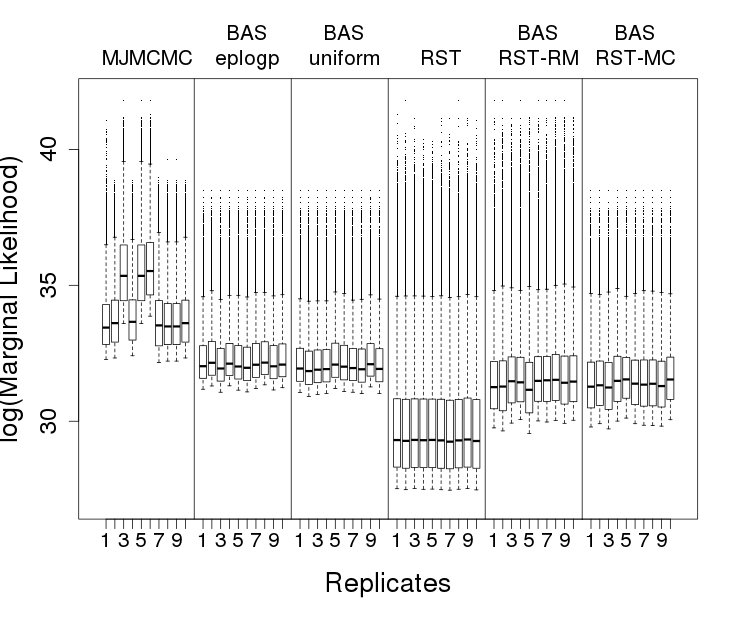
\includegraphics[width=0.48\linewidth]{figures/mliks.jpeg}
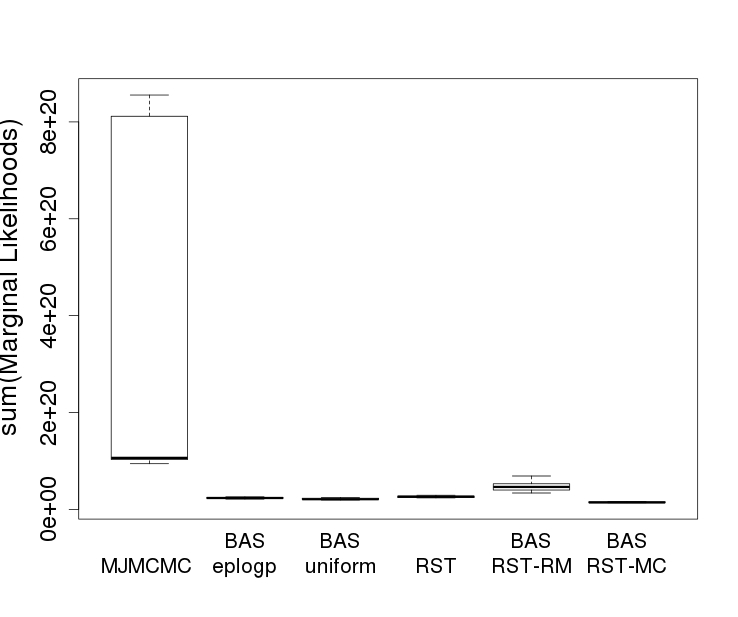
\includegraphics[width=0.48\linewidth]{figures/massesbig.jpeg}\label{figmlikmass}
\captionof{figure}{\color{Black} Comparions of the log marginal likelihood in the protein data of the top 100000 models (left) and boxplots of the posterior mass captured (right) obtained by MJMCMC, BAS-eplogp, BAS-uniform, thinned version of Random Swap (RST), BAS with Monte Carlo estimates of inclusion probabilities from the RST samples (BAS-RST-MC), and BAS renormalized estimates of inclusion probabilities (BAS-RST-RM) from the RST samples.}
\end{center}\vspace{0.2cm}


BAS with both uniform and eplogp initial sampling probabilities perform rather poorly in comparison to other methods, whilst BAS combined with RM approximations from RST as well as MJMCMC show the most promising results. BAS with RM initial sampling probabilities usually manages to find models with the highest MLIK, however MJMCMC in general captures by far higher posterior mass within the same amount of unique models addressed.
%----------------------------------------------------------------------------------------
%	CONCLUSIONS
%----------------------------------------------------------------------------------------

\color{SaddleBrown} % SaddleBrown color for the conclusions to make them stand out

\section*{Conclusions}
\begin{itemize}
\item Novel MJMCMC approach for estimating posterior model probabilities and Bayesian model averaging within GLMM and selection is introduced. 
\item   MJMCMC incorporates the ideas of MCMC with possibility of large jumps combined with local optimizers to generate smart proposals in the discrete space of models
\item \textit{EMJMCMC} R-package is developed and available from the GitHub repository: \url{http://aliaksah.github.io/EMJMCMC2016} -- simply scan the QR code on the top of the poster
\item  The developed package gives a user high flexibility in the choice of methods to obtain marginal likelihoods and model selection criteria within GLMM
\item   Extensive parallel computing for both MCMC moves and local optimizers is available within the developed package
\item Based on the obtained results, MJMCMC can be claimed as a rather competitive novel algorithm in terms of the search quality.
\end{itemize}

\color{DarkSlateGray} % Set the color back to DarkSlateGray for the rest of the content

%----------------------------------------------------------------------------------------
%	FORTHCOMING RESEARCH
%----------------------------------------------------------------------------------------

\section*{Forthcoming Research}

In future it would be of an interest to extend the procedure to the level of selection of link functions, priors and response distributions. The latter is expected to provide new horizons in automation of model selection and thus expand opportunities for addressing properly defined statistical models within machine learning applications. It will also require even more accurate tuning of parameters of the search introducing another important direction for further research.
 %----------------------------------------------------------------------------------------
%	REFERENCES
%----------------------------------------------------------------------------------------
\footnotesize
\color{black}
\let\oldbibliography\thebibliography
\renewcommand{\thebibliography}[1]{\oldbibliography{#1}
\setlength{\itemsep}{2pt}} %Reducing spacing in the bibliography.

\nocite{*} % Print all references regardless of whether they were cited in the poster or not
\bibliographystyle{plain} % Plain referencing style
\bibliography{sample} % Use the example bibliography file sample.bib

%----------------------------------------------------------------------------------------
%	ACKNOWLEDGEMENTS
%----------------------------------------------------------------------------------------
\subsubsection*{Acknowledgements}

\textit{We would like to thank CELS project at the University of Oslo for giving us the opportunity, inspiration and motivation to write this article and Sm\aa forsk project for funding the conference participation.}


%----------------------------------------------------------------------------------------

\end{multicols}
\end{document}